% !TEX TS-program = pdflatex
% !TEX encoding = UTF-8 Unicode

% This is a simple template for a LaTeX document using the "article" class.
% See "book", "report", "letter" for other types of document.

\documentclass[12pt]{article} % use larger type; default would be 10pt
\usepackage[utf8]{inputenc}   % set input encoding (not needed with XeLaTeX)

%%% PAGE DIMENSIONS
\usepackage{geometry}
\geometry{letterpaper}
\geometry{margin=1in} % 1in page margin

%%% COLOR AND GRAPHICS
\usepackage{color}
\usepackage{graphicx} % support the \includegraphics command and options

\usepackage{pslatex}
\definecolor{mygreen}{rgb}{0,0.6,0}
\definecolor{mygray}{rgb}{0.5,0.5,0.5}
\definecolor{mymauve}{rgb}{0.58,0,0.82}
\usepackage{listings} % For displaying source code
\lstset{ %
	language=C,                      % the language of the code
	backgroundcolor=\color{white},   % choose the background color; you must add \usepackage{color} or \usepackage{xcolor}
	basicstyle=\sffamily\fontsize{11}{13.2}\selectfont,        % the size of the fonts that are used for the code
	breakatwhitespace=false,         % sets if automatic breaks should only happen at whitespace
	breaklines=true,                 % sets automatic line breaking
	captionpos=t,                    % sets the caption-position to bottom
	commentstyle=\color{mygreen},    % comment style
	deletekeywords={...},            % if you want to delete keywords from the given language
	escapeinside={\%*}{*)},          % if you want to add LaTeX within your code
	extendedchars=true,              % lets you use non-ASCII characters; for 8-bits encodings only, does not work with UTF-8
	frame=single,                    % adds a frame around the code
	keepspaces=true,                 % keeps spaces in text, useful for keeping indentation of code (possibly needs columns=flexible)
	keywordstyle=\color{blue},       % keyword style
	morekeywords={*,...},            % if you want to add more keywords to the set
	numbers=left,                    % where to put the line-numbers; possible values are (none, left, right)
	numbersep=5pt,                   % how far the line-numbers are from the code
	numberstyle=\color{mygray},      % the style that is used for the line-numbers
	rulecolor=\color{black},         % if not set, the frame-color may be changed on line-breaks within not-black text (e.g. comments (green here))
	showspaces=false,                % show spaces everywhere adding particular underscores; it overrides 'showstringspaces'
	showstringspaces=false,          % underline spaces within strings only
	showtabs=false,                  % show tabs within strings adding particular underscores
	stepnumber=1,                    % the step between two line-numbers. If it's 1, each line will be numbered
	stringstyle=\color{mymauve},     % string literal style
	tabsize=2,                       % sets default tabsize to 2 spaces
	title=\lstname                   % show the filename of files included with \lstinputlisting; also try caption instead of title
}

% \usepackage[parfill]{parskip} % Activate to begin paragraphs with an empty line rather than an indent

%%% PACKAGES
\usepackage{booktabs} % for much better looking tables
\usepackage{array}    % for better arrays (eg matrices) in maths
\usepackage{paralist} % very flexible & customisable lists (eg. enumerate/itemize, etc.)
\usepackage{verbatim} % adds environment for commenting out blocks of text & for better verbatim
%\usepackage{subfig}   % make it possible to include more than one captioned figure/table in a single float
\usepackage{subcaption}
\usepackage{adjustbox}
\usepackage{placeins} % allows for use of \FloatBarrier to prevent floats from moving past line.

%%% HEADERS & FOOTERS
%\usepackage{fancyhdr} % This should be set AFTER setting up the page geometry
%\pagestyle{fancy} % options: empty , plain , fancy
%\renewcommand{\headrulewidth}{0pt} % customise the layout...
%\lhead{}\chead{}\rhead{}
%\lfoot{}\cfoot{\thepage}\rfoot{}


%%% SECTION TITLE APPEARANCE
\usepackage{sectsty}
\sectionfont{\normalsize\bfseries\uppercase}
\subsectionfont{\normalsize\bfseries}
\subsubsectionfont{\normalsize\mdseries\itshape}

%%% ToC (table of contents) APPEARANCE
\usepackage[nottoc,notlof,notlot]{tocbibind} % Put the bibliography in the ToC
\usepackage[titles]{tocloft} % Alter the style of the Table of Contents
\renewcommand{\cftsecfont}{\rmfamily\mdseries\upshape}
\renewcommand{\cftsecpagefont}{\rmfamily\mdseries\upshape} % No bold!

%%% Title setup
\newcommand{\TitleFont}{\fontsize{16}{20}\selectfont\bfseries}
\newcommand{\AuthorFont}{\fontsize{14}{17}\selectfont}

%%% END Article customizations

%%% The "real" document content comes below...

\title{\TitleFont EE 478 Capstone Final Report \\ RFID Interaction Suite \vfill }
\author{\AuthorFont Alyanna Castillo \\ Patrick Ma \\ Ryan McDaniels}
\date{}

\begin{document}

%% Make title and ToC, start page numbering AFTER ToC
\maketitle
\thispagestyle{empty}
\pagebreak \tableofcontents
\listoftables
\listoffigures
\thispagestyle{empty}
\pagebreak
\setcounter{page}{1}

\section{Abstract}
% The abstract should provide a brief overview of the report.  It should provide
% a summary of the main specific points for the introduction, the main tests and
% experiments, the results, and the conclusions. It is called an abstract because
% you can literally "abstract" sentences from the other sections. 
% 
% Once again, this is not a narrative of your experiences as you executed the
% design.  The abstract should mirror (albeit in a very condensed way) the
% content of your report.

\section{Introduction}
% Brief introduction and overview of the purpose of the lab and of the methods
% and tools used.


% This section should include the following:

\textbf{These are some example of how to cite and use bullet points}
A reference to Table~\ref{tab:bomTable} and one to the Design Specification, Section~\ref{sec:designSpec}.

\begin{itemize}
	\item Overall summary description of the module - 2-3 paragraphs maximum
		(explanation of use cases goes here)

		\begin{itemize}
			\item Specification of the public interface to the module

				\begin{itemize}
					\item Inputs
					\item Outputs
					\item Side effects
				\end{itemize}

			\item Psuedo English description of algorithms, functions, or procedures
			\item Timing constraints
			\item Error handling
		\end{itemize}
\end{itemize}


\section{Design Specification}\label{sec:designSpec} 
% In this subsection you will textually describe your client's requirements.
% What does he or she need in the project you are developing.  If you are
% incorporating extra features or capabilities, please describe them clearly in
% this section.

\subsubsection{Design Overview}
This system is a RFID-based gaming system. A user is able to play alone against a computer, or can play with other users owning a system using a multiplayer connection feature. Additionally, users can create their own customized cards using a third built-in function of the device.

\subsection{Design Requirements}\label{sec:requirements} % Patrick , additions by Alyanna, Ryan
\subsubsection{Environmental Requirements}

The device must operate in an indoor/outdoor environment with relative
humidity consistent with desert and tropical environments. It must be durable
enough to withstand various types of users, especially small children.  The
unit is to be portable and battery operated.

\subsubsection{System Input and Output Requirements}

The system must be capable of accepting several different types of signals and
inputs:

\begin{itemize}
	\item Standard frequencies used for close-range or Near-Field Communication
		Radio Frequency Identification (RFID) devices
	\item Standard frequencies used for commercial wireless communication
		standards such as wifi networks
	\item User input from a keypad to navigate menus, enter commands, and provide
		other alphanumeric information
	\item When in multiplayer mode, communication and commands from other players
		must be accepted and responded to.
\end{itemize}

The system must be capable of providing the following outputs:
\begin{itemize}
	\item Display information about the current game state through an LCD screen
	\item Provide status information of individual cards placed on the game board
	\item Send commands to other systems when in multiplayer mode
	\item Send wireless signals to program RFID-enabled cards
\end{itemize}

\subsubsection{User Interface}

The system must also have the following buttons, switches or interface devices:

\begin{itemize}
	\item 16-button keypad with alphanumeric character labels
	\item Reset button that when pressed causes a soft reset of the system
	\item Power button that turns the system on and off
	\item An LCD screen viewable from several angles. The screen must be viewable indoors and in overcast conditions
\end{itemize}

An example User interface is shown in Figure~\ref{fig:exampleFrontPanel}.

\begin{figure}[h]
	\centering
	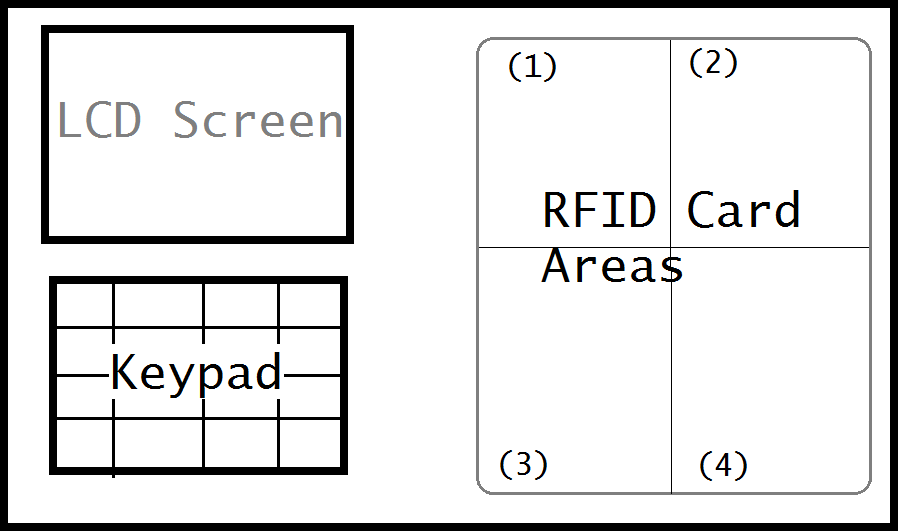
\includegraphics[width=0.6\textwidth]{images/exampleFrontPanel.png}
	\caption{An example front panel layout for the system}
	\label{fig:exampleFrontPanel}
\end{figure}

\subsubsection{Functional Requirement}

The system must support the following modes of operation:

\begin{description}
	\item[Single Player:] Allows the user to select from, and play, single player
		games. Upon entering Single Player mode, the system prompts the user to
		select a game to play from those stored in memory. Selecting a valid game
		loads the game from memory and begins game execution.
	\item[Multiplayer:] Allows the user to select and play multiplayer games.
		Upon entering Multiplayer mode, the system activates wireless communication
		and attempts to connect to other users in Multiplayer mode. Once a
		connection is established, the users select a multiplayer game on both
		systems and gameplay begins.
	\item[Build Card:] Allows the user to create custom cards for a game. To
		create a custom card, the user will input the data via the keypad. The data
		stored will vary based on game requirements. All cards must contain unique
		card serial numbers or identifing ID numbers, and a code that specifies
		which games the card is valid for.
\end{description}

In all three modes, the user will be instructed by the programmed game to place
a card in the RFID reading area to interact with the game and control events. 

\subsubsection{Operating Requirements}

The system must operate in a standard commercial or household environment. The system must be portable, wearable on the user's arm, and operate on an internal power supply.

\subsubsection{Reliablility and Safety Requirements}

The system must be compliance with communication and electromagnetic radiation
standards including those from the U.S. Federal Communication Committee, and
applicable state and federal child safety laws.

\subsection{Identified Use Cases}\label{sec:identifiedUseCases} % Alyanna

The user interacted with the system through the game. In the figure below, a user would interact with the system through single player,
multiplayer, or build card mode. In a single player game, the user would play against a computer. In a build card game, the user would be working
with the system to create/modify cards. Should a user be in multiplayer mode, they would interact with another using using the system during gameplay.

\subsection{Detailed Specifications}\label{detailedSpec} % Ryan
\subsubsection{System Description}\label{designSystemSpec}

This specification describes and defines the basic requirements for a wearable digital card-gaming device. The device will house 1 DLP-RFID2 reader module that will take data from RFID cards. As cards are placed on the device, a 4-inch linear servo will move the reader to scan each card and use it in a game of the user’s choosing. The user has the option of doing a single player, multiplayer, or build their own card deck. In multiplayer mode, the user would be able to wirelessly communicate with one other player in possession of another device via the Xbee wireless module.

\subsubsection{Specification of External Environment}\label{designExtEnv}
The device is to be operated in an indoor/outdoor environment with relative humidity consistent with desert and tropical environments. It must be durable enough to withstand various types of users, especially small children.  The unit is to be portable and battery operated.

\begin{description}
	\item[Temperature Range:] 0-60C (32-140F)
	\item[Humidity:] Humidity 30-60% non-condensing
\end{description}

\subsubsection{System Inputs}\label{inputs}
The system must support the measurement of the following kinds of signals:

\begin{itemize}
	\item Frequency in the standard 13.56 MHz range for close range RFID signals
	\item Frequency in the 2.4 GHz range for wireless communication with Xbee modules
	\item It will follow protocols from ISO 15693 for RFIDs
	\item User input via the 16-character keypad.
\end{itemize}

Reading of RFID cards will be done by sending standard control strings, such as “0108000304FF0000” (for “ping”) to the DLP-RFID2.  These strings will allow control over read and write functions on the device.  These strings will be programmed into a driver on a microcontroller.  Each RFID tag will have an identifier so that its information can be looked up in the system’s memory.   These strings are sent through a 115200 baud UART connection and are detailed in Table~\ref{Tab:DLP RFID-2 input commands}.

\begin{table}[h]
	\begin{tabular}{ll}
		\multicolumn{2}{c}{\textbf{DLP RFID-2 Commands}}                                     \\
		\textbf{Description}                & \textbf{String}                                \\
		Inventory (Find cards in range)     & 010B000304140601000000                         \\
		Set data in/out to user memory      & 010C00030410002101020000                       \\
		AGC mode (Alternating Gain Control) & 0109000304F0000000                             \\
		Write to block                      & 0113000304182220{[}UID{]}{[}BLOCK{]}{[}DATA{]} \\
		Read block                          & 0117000304186221                              
	\end{tabular}
	\caption{Command strings to control the RFID reader.}
	\label{Tab:DLP RFID-2 input commands}
\end{table}

The system will also accept user input from a keypad that will determine which mode to set the game in: single player, multiplayer, or card building. It will also allow the user to navigate the menu screens and select their next move. The controls for navigation can be found in Table~\ref{Tab:controlsTable}.

\begin{table}[h]
	\begin{tabular}{ll}
		\multicolumn{2}{c}{\textbf{User Keypad Input}} \\
		\textbf{Command}         & \textbf{Key}        \\
		Move Up                  & 2                   \\
		Move Down                & 8                   \\
		Move Left                & 4                   \\
		Move Right               & 6                   \\
		Select/Enter             & D                   \\
		Back/Return              & B                  
	\end{tabular}
	\caption{Controls to navigate through the system's menus.}
	\label{Tab:controlsTable}
\end{table}

If the system is in multiplayer mode, it must receive game data from the device of another player and modify the user's game state based on that data. The shared data consists of players’ scores, current cards on the field, etc.

The connection between two systems must be implement the IEEE 802.15.4 wireless networking protocol. To identify potential connections, the system must send a “ping” command followed by a unique system identification number (a serial number). The system then waits three seconds for any response. If no valid response occurs, the system recommences the search sequence up to five times. A system responding to a connection request waits until the connection request ends then sends the ID of the system it wishes to connect followed by its own system ID. The system then waits for confirmation of the request from the other system. During game play, the system sending data transmits the ID of the second system's Xbee, followed by the data.

\subsubsection{System Outputs}\label{outputs}

The system must display information about the current game state and the reading from the RFID signal on an LCD display.  The display will show a menu that will allow a user to navigate through options using a keypad.  When a game is being played, the display will show information relevant to the game, such as simple graphics, scores, instructions, and player moves.

The system will respond to cards being placed in the card reader area.  The card will be physically “locked in” until the user decides to place another card in its place.  An LED will also indicate that a card has been correctly placed and read, according to Table~\ref{Tab:LEDTable}.

\begin{table}[h]
	\begin{tabular}{ll}
		\multicolumn{2}{c}{\textbf{LED Color Indications}} \\
		\textbf{Card Status}           & \textbf{Color}    \\
		Card placed and recognized     & Green             \\
		Card placed, not read          & Yellow            \\
		Error reading card             & Red               \\
		No card placed                 & Off              
	\end{tabular}
	\caption{Status of LED lights based on RFID read state}
	\label{Tab:LEDTable}
\end{table}

When the system is in multiplayer mode, data must be sent wirelessly to another device. This data consists of players’ scores, current cards in play for the game, etc.  The LCD display will show information about the second player, like player name, in addition to information relevant to the game. 

\subsubsection{User Interface}\label{UI}

The user must be able to select the following using the keypad on the front panel of the instrument:

\begin{itemize}
	\item Mode
		\begin{itemize}
			\item Singleplayer
			\item Multiplayer
			\item Build Cards
		\end{itemize}
	\item Card Reader
		\begin{itemize}
			\item Physical space to place cards
		\end{itemize}
\end{itemize}

Game mode can be selected through a menu screen on the LCD display – the user will be able to navigate the menu with a keypad. Similar to a gaming device, the power will be controlled by a switch and reset will be a push button. Game output will be displayed on an LCD display.  Such a display must be readable from several angles.  The front panel of the system can be found in Figure~\ref{fig:exampleFrontPanel}.

\subsubsection{System Functional Description}\label{sysFunctDesc}

A user will be provided with a deck of RFID cards that contain data about whatever game the user wants to play.  These cards would be used in the RFID reading device that would be worn by the user on their arm.  First, the user must choose using the keypad what game mode they would like to play: single player, multiplayer, or card building.  In all three modes, the user will be instructed by the programmed game to place a card in the RFID reading area to interact with the game and control events. In multiplayer mode the user would have to find the other user they would like to play with and connect to their game using the wireless features of the system.  In card building mode, the user would be able to enter data via the keypad to program their own data onto whichever RFID card they choose.  A block diagram for the system can be found in Figure~\ref{fig:highLevelBlockDiagram}.  The system functionality is described below.

\begin{itemize}
	\item Read/Write Cards: 
		\begin{itemize}
			\item Communicate w/ DLP: The chosen RFID reader is the DLP-RFID2 reader/writer module. The system must communicate with this reader using the RS-232 protocol at TTL voltage levels. The communication link must be at 115200 Baud, 8-bits, 1 stop bit, and no parity check. The commands to the RFID reader are specified in TRF7960_ISO15693_protocol.pdf 
			\item Traverse card data: The system must read up to five cards
			\item Quantity of Cards: The Reader must be able to read and write to 5 cards at a time.
			\item Write Card: Data must be written to the card according to the ISO 15693 standard. The structure of data contained on the card may vary with the game associated with the card. The following data locations must be present:
				\begin{itemize}
					\item Unique card Identifier (UID) – A serial number uniquely identifying the card from all other cards
					\item Card name – The name of the card
					\item Display name – The name of the card as displayed to the user
					\item Associated Programs – A code that identifies the card as valid for a specific game set.
				\end{itemize}
			\end{itemize}
	\item Access Database
		\begin{itemize}
			\item Read Data to SRAM: The system must be capable of requesting data from the SRAM using a byte-addressing scheme. The returned data must be received as an 8-bit word in parallel.
			\item Write data to SRAM: The system must be capable of requesting data from the SRAM using a byte-scheme. Data must be sent as an 8-bit word in parallel.
			\item Lookup/reference Table:
		\end{itemize}
	\item User Interaction
		\begin{itemize}
			\item Read Keypad: The system must read user keypad input with a maximum lag time of 250 ms.  
			\item Display: The system must display the following
				\begin{itemize}		
					\item Simple graphics
					\item Score
					\item Game instructions
					\item Player options
				\end{itemize}
			\item Card Reactions: When a card is placed on the reader, the system must acknowledge the card through a series of LEDs. If the card is read/accepted as valid, green appears. If the card cannot be read, red appears. Additional colors may indicate other statuses
\item External Communications (ExtCom): 
a.	Xbee: The system must be capable of maintaining a connection with another system using the XBee wireless standard over a minimum distance of 5 feet. Data transmission must occur at 250kbs. 
b.	RS-232 connection: The system must be capable of maintaining an EIA-232 serial connection with an external computer system. Data sent must be at 9600 baud, 8-bit, 1-stop bit, and no priority.
c.	Wireless Driver: The driver must be capable of sending commands to initiate connections, acknowledge received data, sending data, and terminating a connection
d.	RS-232 Driver: The driver must be capable of sending strings of data up to 20 characters in length. The encoding must use the extended ASCII table.
\end{itemize}

 
\subsection{Functional Decomposition}\label{functions} % Patrick

\section{Hardware Implementation}\label{hwImplementation} 

\subsection{Top Level Design}\label{hwTopLevel} % Patrick

\subsection{Low Level Design}\label{hwLowLevel} % Patrick

\section{Software Implementation}\label{swImplementation}
%
%What is your design????
%
%Present your design starting from a top level functional view and potentially
%block diagram or high level architecture.  Refine that view to present and
%explain each of the modules that comprise the major functional blocks.
%Discuss
%the flow of control through the design.  Identify and discuss the specific
%processes/tasks you have implemented in your design. Explain your design
%choices.    

\subsection{Top Level Design}\label{swTopLevel} % Alyanna
%
%Put stuff here about the functional decomposition, system architecture,
%interaction of parts.

The software implementation for the RFID interaction suite consisted of developing the game for a user to play \(and for the developers to test\). The system took input from the Xbee, RFID tags, and keyboard. Data would be outputted through the LCD screen. Below is a figure depicting the overall software for the RFID interaction suite. 

\begin{figure}[H]
	\centering
	\includegraphics[width=\textwidth]{images/funDecomp.png}
	\caption{Software functional decomposition showing the major functional divisions and tasks}
	\label{fig:funDecomp}
\end{figure}

\begin{itemize}
	\item Play Game
		\begin{itemize}
			\item Load Game: The program would have to load the correct game based off of user input through the keypad. The system is told which game to select based off of a set flag.
			\item Execute Game: After a game flag has been set, the game would run until a player has finished.
		\end{itemize}
	\item Read/Write Cards
		\begin(itemize)
			\item Scan for New Cards: During game mode or build card mode, the system would scan for new cards via the RFID reader/writer.
			\item Write Card: During the "build card" part of the game, the user would be able to write data to the cards through the RFID reader/writer. The user would have the ability to add a name and attack moves to the card through the external keypad and the in-game keyboard.
			\item Read card: During game mode, the system would check for available cards to work with. If a player was in the middle of a duel, the system would scan for new cards to use for gameplay. If a reader was trying to build new cards, the system would look for available cards to be modified.
		\end(itemize)
	\item Access Database
		\begin(itemize)
			\item Read Data to SRAM: Reads game-relevent data. For example, when a game is to be loaded, the system load the game from the SRAM. Or if the computer were to read in a monster during a single player duel game, it would access the database of monsters.
			\item Write Data to SRAM: Writes new game data. If new monsters or games were to be added to the system, it would be written to the SRAM for future use.
			\item Look Up / Reference Table: Used as a reference for memory locations of data in the SRAM \(i.e. ''Phone book''\).
		\end(itemize)
	\item External Communication
		\begin(itemize)
			\item RS232 Driver: The back end of the system uses the USART to communicate with the Xbee wireless chips and RFID drivers. Information was sent out or recieved by the system through these peripherals.
			\item Wireless Driver: In addition to the RS232, a driver for the Xbee wireless had to be implemented to allow the system to communicate with other users during the multiplayer game.
		\end(itemize)	
	\item User Interaction
		\begin(itemize)
			\item Read Keypad: A driver was made to read key presses from the user. Different parts of the system could read the keypad using functions built in this driver.
			\item Display: An LCD driver was modified to develo
			\item Card Reaction: An LED driver was made to control the LED lights of the RFID interaction suite. This would indicate to the user whether a card had been properly registered or not, based off of the color of the lights.
		\end(itemize)
\end{itemize}


\subsection{Low Level Design}\label{swLowLevel} % Alyanna
%
%task level implementation details here. Control diagram goes here, etc.



A major software component of the RFID interaction suite were the built in games.

\begin{itemize}
	\item LCD.c and LCD.h
		\item The majority of documentation for our ST7735 1.8 TFT LCD screen did not include example code for how to use the screen. Most tutorials or example code \(i.e. Adafruit\) assumed that the user would be programming on an Arduino UNO, which had built in libraries for fonts and shapes. The link below features code found on Google which interfaces the LCD with a PIC microcontroller using the chip's SPI function. However the code was not optomized, thus LCD.c and LCD.h are modified versions of the code. The original drawBox function in LCD.c created a box pixel by pixel - it would take a beginning pixel location and an ending pixel location, causing load times to take longer. The new box function takes the beginning and end coordinates for the box and fills everything in between by printing out pixels all at once. Another function printrs was made to take a char pointer to a string and print it out on the LCD. A major advantage to using this example code was that it already built a font library for the LCD screen. Had the group not utilized this, they would have taken time defining the pixel structure for every possible character. 
		\item Original Code (unmodified): https://sites.google.com/site/arduinomega2560projects/microchip-pic/level-3/st7735-1-8-tft
	\end {itemize}

% Insert State Machine for Game Here	
	
\begin{itemize}
	\item Game.c and Game.h
		\begin{itemize}
			\item Single Player: Single player mode followed the direction of the state machine diagram. All random variables were seeded to a system timer on the PIC.
			\item Multiplayer:
			\item Build Cards: 
		\end{itemize}
\end{itemize}

\begin{itemize}
	\item Multiplayer Game
		\begin{itemize}
			\item Specification of the public interface to the module

				\begin{itemize}
					\item Inputs
					\item Outputs
					\item Side effects
				\end{itemize}

			\item Psuedo English description of algorithms, functions, or procedures
			\item Timing constraints
			\item Error handling
		\end{itemize}
\end{itemize}

\begin{itemize}
	\item Build Card Game

		\begin{itemize}
			\item Specification of the public interface to the module

				\begin{itemize}
					\item Inputs
					\item Outputs
					\item Side effects
				\end{itemize}

			\item Psuedo English description of algorithms, functions, or procedures
			\item Timing constraints
			\item Error handling
		\end{itemize}
\end{itemize}

\section{Presentation, Discussion, and Analysis of the Results}
%
%Based upon the execution of your design, present your results. Explain them
%and
%what was expected, and draw any conclusions (for example, did this prove your
%design worked).
%
%In addition to a detailed discussion and analysis of your project and your
%results, you must include all the answers to all questions raised in the lab.
\subsection{Results } % Ryan

\subsection{Discussion of Results } % Alyanna

\subsection{Analysis of Any Errors } % Ryan
%
%This one is obvious. Do this section as appropriate.  If it improves the flow,
%it does not need to be a separate section and may be included in the
%presentation, discussion, and analysis of the results.  However, it will still
%be graded separately and must be present.

The biggest problem with the final version of this project that was present at
demo time was the fact that the multiplayer features were not implemented.
There was test code that correctly configured the Xbee modules for multiplayer,
but they were not completely implemented with the game.  The reason for this
was because when the $I^2C$ system was implemented, the entire game had to be
modified to run within the scheduler, when it was just a single function
before.  $I^2C$ communication is controlled by the system's interrupt handler,
and certain flags are set depending on whether data is being sent or received.
Those flags have to be processed, and a game that is running in a function and
taking control of the entire system would not allow for those flags to be
processed.  The time it took to port the game over to running completely within
the scheduler made it impossible to get the multiplayer functions completely
implemented and working in time.

Another problem at the time of the demo was that card reading was not 100\%
functional.  The system had four distinct sets of data that could be
successfully written to a card using the ``Build Cards'' option from the
system's main menu, but the data was not being displayed properly in the
singleplayer game.  Data coming from the card over the $I^2C$ connection was
confirmed to be correct, but the game was not interpreting and displaying the
information correctly to the user.  This was also a matter of running out of
time.  For the same reasons as above (converting the game to be run within the
flag-based scheduler) the RFID reading still had some kinks to work out at the
time of the demo.  Those problems were that:

\begin{itemize}
	\item Monster type was being read incorrectly
	\item Monster name was being displayed incorrectly
	\item Complete attack list was not implemented
\end{itemize}

For demo purposes, only the first attack would be read and it would be copied
to all three attack slots.  Only the ``FAIL'' attack ID was programmed to be
read, and if the ID did not match the ``FAIL'' attack's ID, then it was
interpreted as a ``SCRATCH'' attack.  This function worked correctly, but the
rest of the attack IDs were not implemented.  The monster's level was correctly
read as well.

Finally, there was an error when finishing a singleplayer game.  When the game
was complete, the main menu was not being properly displayed.  Once again, the
problem was time, and the main menu's controls were still functional.  Another
menu could be loaded by navigating the invisible menu and choosing an option,
letting that screen load, and then pressing the ``B'' key to return back to the
main menu and redraw it.

\subsection{Analysis of Implementation Issues and Workarounds} % Patrick
%
%State any problems you encountered while working on the project. If your
%project did not work or worked only partially, provide an analysis of why and
%what efforts were made to identify the root cause of any problems. \\
%

\section{Test Plan } % Ryan
%
%Overall summary of what needs to be tested to ensure that your design meets
%the
%original requirements, 2-3 paragraphs maximum unless specified otherwise

\subsection{Test Specification} % Patrick
%
%Annotated description of what is to be tested and the test limits.  This
%specification quantifies inputs, outputs, and constraints on the system.  That
%is, it provides specific values for each. 
%
%Note, this does not specify test implementation...this is what to do, not how
%to do it.

\subsection{Test Cases} % Alyanna
%
%Annotated description of how your system is to be tested against the test
%limits
%Note, this does specify test implementation...this is not what to do, this is
%how to do it based upon the test specification.




\section{Summary and Conclusion}
%
%You should know these sections very well, no need to explain.  Note, however,
%that they are two different sections.  The summary is just that, a summary of
%your project.  It should loosely mirror the abstract with a bit more detail.
%The conclusion concludes the report, potentially adds information that is
%often
%outside the main thrust of the report, and may offer suggestions or
%recommendations about the project.

\subsection{Final Summary}


\subsection{Project Conclusions} % Patrick, Alyanna, Ryan
% Include comments and reflections on the capstone. What went well, what could
% be improved next time, What was enjoyable and/or challenging.

This project had many hardware components that were new to the group. There was little documentation to gooff of and previous capstone projects had not done anything similar to our design requirements. Much of the project was spent
reading documentation and figuring out how to design drivers compatible with the PICs, since most available documentation was
for Arduinio shields. Using the LCD and Xbee was more difficult since online tutorials referenced the Arduino shield. RFID tags
were a completely new piece of hardware to work with with little documentation that the group had to contact the company for help.

With all this new technology, the group broke down building and testing into separate components. The intention was to put everything
together at the end and make a scheduler to fire off every function at a particular time. This was the first development flaw - assuming
everything would work when put together. There was miscommunication over how the scheduler would work that many functions with while 
loops had to be redone using flags. A better method would have been to consistently putting components together once their functionality
was verified separately. Additionally, another PICKit 3 should have been bought for use during testing - with only one PICKit, components
had to be tested and debugged one at a time after programming. The ability to consistently load the program into PICs and observe the results
would have reduced the time for debugging and testing each individual part.

The original intent of the project was to have a working motor that would move the
RFID reader to read multiple cards. Another feature was that he user would also be able to make custom cards
with their own ID, attack names, moves, and type. Due to time constraints and testing, these idea had
to be scrapped in the final implementation. Future implementations should include these features.

\pagebreak
\appendix


\section{Breakdown of Lab Person-hours (Estimated)}
% Use the '&' to separate columns
\begin{tabular}{|l|*{4}{r|}}
	\hline
	Person & Design Hrs & Code Hrs & Test/Debug Hrs & Documentation Hrs \\ \hline
	Patrick & x & x & x & x  \\ \hline
	Alyanna & x & x & x & x \\ \hline
	Ryan & x & x & x & x  \\ \hline
\end{tabular}

~\\

By initializing/signing above, I attest that I did in fact work the
estimated number of hours stated. I also attest, under penalty of shame,
that the work produced during the lab and contained herein is actually my
own (as far as I know to be true). If special considerations or
dispensations are due others or myself, I have indicated them below.

\pagebreak

\section{Bill of Materials\label{appendix:bom}}
Table~\ref{tab:bomTable} lists the bill of materials for the construction of
one system.

\begin{table}[h]
	\begin{tabular}{llll}
		\multicolumn{4} {c} {\textbf{Bill of Materials}} \\
		\toprule
		\textbf{Item}                         & \textbf{Unit Cost} & \textbf{Quantity} & \textbf{Total Cost} \\ \midrule
		TI HI-Plus RFID Tags                  & 0.91          & 20                & 18.20               \\
		DLP-RFID2 RFID Reader/Writer          & 50            & 3                 & 150                 \\
		Xbee S1 Wireless Chips                & 30            & 2                 & 60                  \\
		PLA Makerbot Filament                 & 48            & 1                 & 48                  \\
		GAL22V10D                             & 3.5           & 4                 & 14                  \\
		PICKit 3                              & 45            & 2                 & 90                  \\
		CY7C128A SRAM                         & 4             & 2                 & 8                   \\
		3.3 Volt Linear Regulator             & 3.22          & 2                 & 6.44                \\
		Lever Switch, micro SPDT, momentary   & 2.5           & 6                 & 15                  \\
		16-key Numeric Keypad                 & 7.5           & 2                 & 15                  \\
		128x169 Color LCD                     & 17            & 2                 & 34                  \\
		PIC18F46K22 Microcontrollers          & 7.7           & 4                 & 30.8                \\
		RGB LED, Common Cathode               & 4             & 8                 & 12                  \\
		(EXTRA)                               &               &                   &                     \\
		(EXTRA)                               &               &                   &                     \\
		(EXTRA)                               &               &                   &                     \\ \bottomrule
		Total Cost                            &               &                   &                    
	\end{tabular}
	\caption{\label{tab:bomTable}}
\end{table}

%\FloatBarrier
%\section{Hardware Diagrams\label{appendix:hwDiagrams}}
%\begin{figure}[H]
%	\centering
%	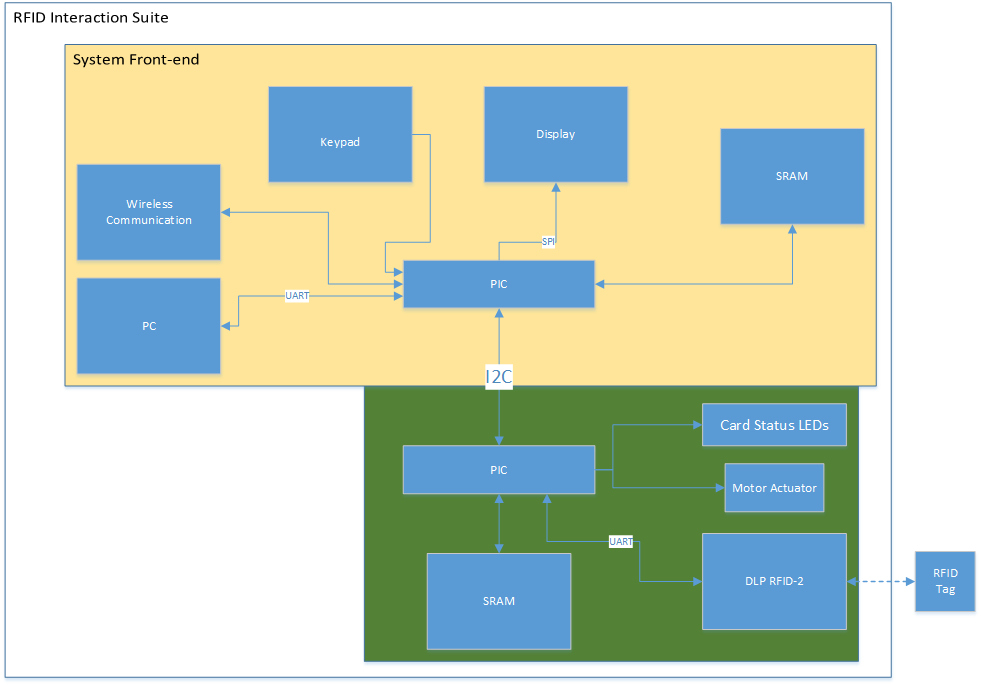
\includegraphics[width=\textwidth]{images/BlockDiagram.png}
%	\caption{High level block diagram of the system hardware components}
%	\label{fig:highLevelBlockDiagram}
%\end{figure}
%
%\begin{figure}[H]
%	\centering
%	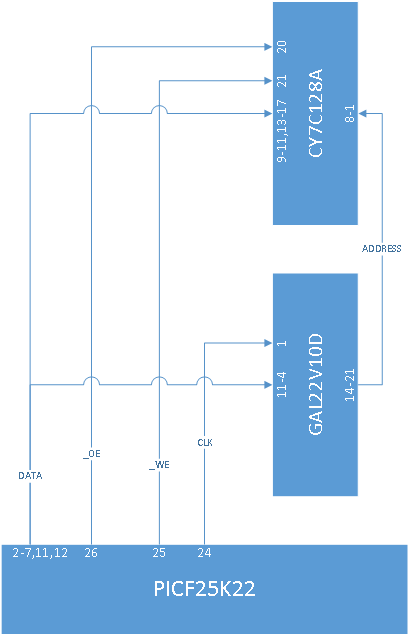
\includegraphics[width=0.8\textwidth]{images/SRAMHardwareBlock.png}
%	\caption{Block diagram of the SRAM hardware system}
%	\label{fig:sramBlockDiagram}
%\end{figure}
%
%\begin{figure}[H]
%	\centering
%	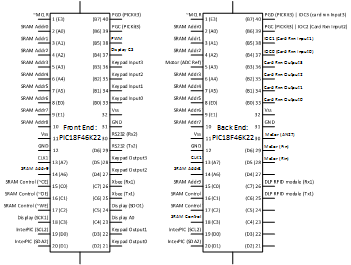
\includegraphics[height=4in]{images/PinOuts.png}
%	\caption{Pinouts to the front- and back-end microcontrollers}
%	\label{fig:pinoutDiagram}
%\end{figure}
%
%\FloatBarrier
%\section{Functional Decomposition Diagram\label{fig:funcDecomp}}
%
%\begin{figure}[H]
%	\centering
%	\includegraphics[width=\textwidth]{images/funDecomp.png}
%	\caption{Software functional decomposition showing the major functional
%	divisions and tasks}
%	\label{fig:funDecomp}
%\end{figure}
%
%\FloatBarrier
%\section{State Diagrams}
%\FloatBarrier
%\subsection{System State Diagram\label{fig:sysStateDiagram}}
%\begin{figure}[H]
%	\centering
%	\begin{subfigure}{0.48\textwidth}
%		\includegraphics[width=\textwidth]{images/overallSystemDiagram.png}
%		\caption{}
%		\label{fig:sysStates}
%	\end{subfigure}
%	~
%	\begin{subfigure}{0.48\textwidth}
%		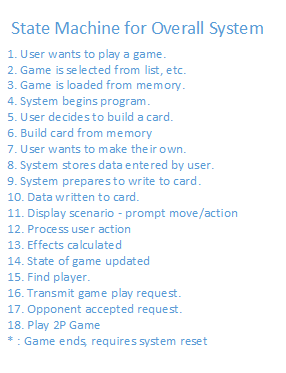
\includegraphics[width=\textwidth]{images/OSStates.png}
%		\caption{}
%		\label{fig:statesLegend}
%	\end{subfigure}
%	\caption{State diagram of the primary operating system.
%		Figure~\ref{fig:sysStates} shows the states while
%		Figure~\ref{fig:statesLegend} provides a legend}
%		\label{fig:systemStateDiagram}
%	\end{figure}
%
%	\FloatBarrier
%	\subsection{General Gameplay State Diagram\label{appendix:gameplayDiagram}}
%	\begin{figure}[H]
%		\centering
%		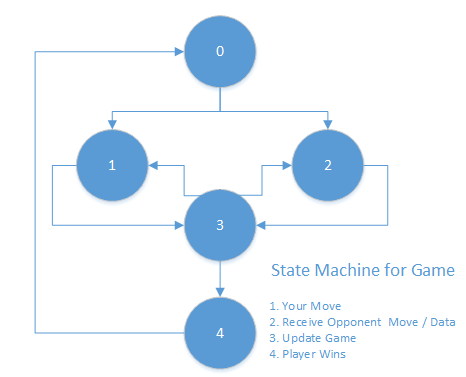
\includegraphics[width=\textwidth]{images/gamePlayState.png}
%		\caption{State diagram of basic turn-based game}
%		\label{fig:gamePlayState}
%	\end{figure}
%
%	\FloatBarrier
%	\section{Control Flow Diagrams}
%
%	\begin{figure}[H]
%		\centering
%		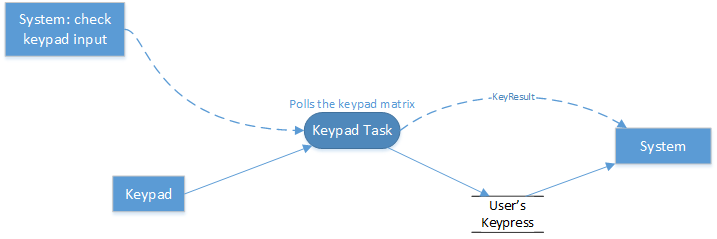
\includegraphics[width=0.75\textwidth]{images/keypadDataFlow.png}
%		\caption{Keypad response}
%		\label{fig:keypadDataFlow}
%	\end{figure}
%
%	\begin{figure}[H]
%		\centering
%		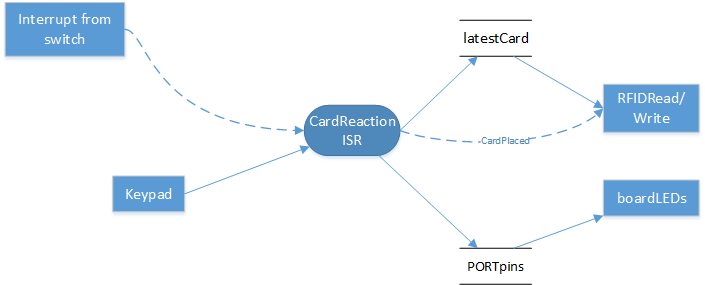
\includegraphics[width=0.8\textwidth]{images/reactionDataFlow.png}
%		\caption{Card Reaction LEDs}
%		\label{fig:cardReactionDataFlow}
%	\end{figure}
%
%	\begin{figure}[H]
%		\centering
%		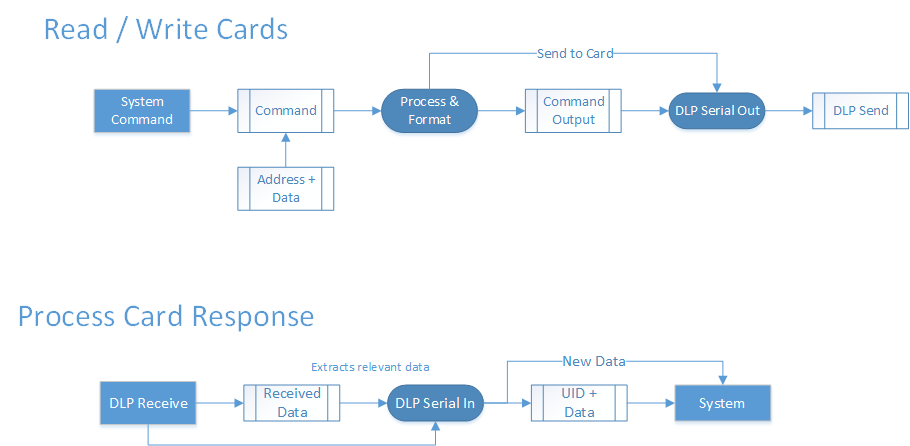
\includegraphics[width=0.8\textwidth]{images/RFIDreaderDataFlow.png}
%		\caption{RFID tag reader subsystem}
%		\label{fig:rfidDataFlow}
%	\end{figure}
%
%	\begin{figure}[H]
%		\centering
%		\begin{subfigure}{\textwidth}
%			\includegraphics[width=\textwidth]{images/I2CReceiveDataCtrlFlow.png}
%			\caption{}
%			\label{fig:i2cReceiveFlow}
%		\end{subfigure}
%
%		\begin{subfigure}{\textwidth}
%			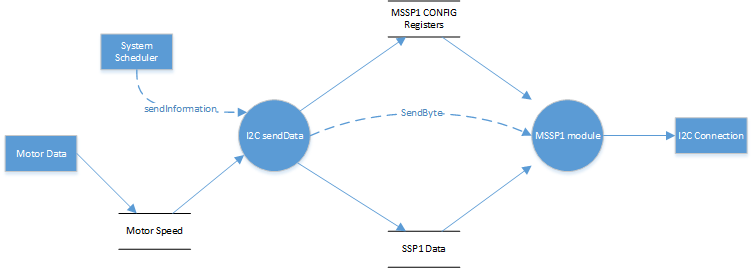
\includegraphics[width=\textwidth]{images/I2CSendCtrlFlow.png}
%			\caption{}
%			\label{fig:i2cSendFlow}
%		\end{subfigure}
%		\caption{I2C communication between microcontrollers.
%		Figure~\ref{fig:i2cReceiveFlow} shows the flow for received data and
%		Figure~\ref{fig:i2cSendFlow} shows the flow for transmitted data.}
%		\label{fig:i2cCtrlFlow}
%	\end{figure}
%
%	\FloatBarrier
%	\section{Project Schedule\label{appendix:ganttChart}}
%	\begin{figure}[h]
%		\centering
%		\begin{adjustbox} {rotate=90,center}
% 		
\includegraphics[height=0.7\textwidth]{images/NewGantt.png}
% 	\end{adjustbox}
% 	\caption{Project Gantt Chart}
% 	\label{fig:ganttChart}
% \end{figure}
%
%	\clearpage
%	\section{Source Code}
% We will put code here. Use the format:
%    \subsection{Main Function}
%%    \lstinputlisting{../code/main.c}
%%
%%    \subsection{Tasks}
%%    \subsubsection{Task Control Blocks}
%%    \lstinputlisting{../code/tcb.h}
%	Source code for this project is provided below.
%
%	\subsection{System Scheduler}
%	The system-wide global definitions and variables are also given here for
%	convenience.
%	\lstinputlisting{../FrontEnd.X/globals.h}
%	\lstinputlisting{../FrontEnd.X/interrupts.h}
%	\lstinputlisting{../FrontEnd.X/SchedMain.c}
%
%	\subsection{Creating Cards}
%	\lstinputlisting{../FrontEnd.X/buildCard.c}
%
%	\subsection{Example Game}
%	Both a single player and multiplayer version of the same game are provided.
%	\lstinputlisting{../FrontEnd.X/game.h}
%	\lstinputlisting{../FrontEnd.X/game.c}
%
%	\subsection{I$^2$C InterPIC Communication}
%	\lstinputlisting{../FrontEnd.X/i2cComm.h}
%	\lstinputlisting{../FrontEnd.X/i2cComm.c}
%
%	\subsection{Keypad Driver}
%	\lstinputlisting{../FrontEnd.X/keypadDriver.h}
%	\lstinputlisting{../FrontEnd.X/keypadDriver.c}
%
%	\subsection{LCD Driver}
%	\lstinputlisting{../FrontEnd.X/LCD.h}
%	\lstinputlisting{../FrontEnd.X/LCD.c}
%
%	\subsection{Card Reaction Control}
%	\lstinputlisting{../FrontEnd.X/LED.h}
%	\lstinputlisting{../FrontEnd.X/LED.c}
%
%	\subsection{Motor Driver}
%	\textit{Note: This feature was not implemented in the final product}
%	\lstinputlisting{../FrontEnd.X/motorDriver.h}
%	\lstinputlisting{../FrontEnd.X/motorDriver.c}
%
%	\subsection{RFID Reader Driver}
%	\lstinputlisting{../FrontEnd.X/rfidReader.h}
%	\lstinputlisting{../FrontEnd.X/rfidReader.c}
%
%	\subsection{EIA-232 Serial Connection}
%	\lstinputlisting{../FrontEnd.X/rs232.h}
%	\lstinputlisting{../FrontEnd.X/rs232.c}
%
%	\subsection{SRAM Primary Memory}
%	\textit{Note: There are two different files for each microcontroller due to
%	hardware configurations}
%	\lstinputlisting{../FrontEnd.X/SRAM.h}
%	\lstinputlisting{../FrontEnd.X/SRAMfront.c}
%	\lstinputlisting{../FrontEnd.X/SRAMback.c}
%
%	\subsection{SPI Initialization}
%	\textit{Note: SPI used for communication with the LCD display}
%	\lstinputlisting{../FrontEnd.X/startup.h}
%	\lstinputlisting{../FrontEnd.X/startup.c}
%
%	\subsection{Wireless Connectivity via Xbee}
%	\lstinputlisting{../FrontEnd.X/xbee.h}
%	\lstinputlisting{../FrontEnd.X/xbee.c}
%
	\end{document}
